\documentclass[output=book
		,modfonts
		,nonflat
	        ,collection
	        ,collectionchapter
	        ,collectiontoclongg
 	        ,biblatex  
                ,babelshorthands
%                ,showindex
                ,newtxmath
                ,colorlinks, citecolor=brown 
                ,draftmode
% 	        ,coverus
		  ]{./langsci/langscibook}                              
%%%%%%%%%%%%%%%%%%%%%%%%%%%%%%%%%%%%%%%%%%%%%%%%%%%%

% put all additional commands you need in the 
% following files. If you do not know what this might 
% mean, you can safely ignore this section

\title{Head-Driven Phrase Structure Grammar}  %look no further, you can change those things right here.
\subtitle{The handbook}
% \BackTitle{Change your backtitle in localmetadata.tex} % Change if BackTitle != Title
\BackBody{Head-Driven Phrase Structure Grammar (HPSG) is a linguistic framework that models
  linguistic knowledge on all descriptive levels (phonology, morphology, syntax, semantics,
  pragmatics) by using feature value pairs, structure sharing, and relational constraints. This
  volume summarizes work that has been done since the mid 80s. Various chapters discus formal foundations and
  basic assumptions, describe the evolution of the framework and go into the details of various
  syntactic phenomena. Separate chapters are devoted to non-syntactic levels of description. The
  book also handles related fields and research areas (gesture, sign languages, computational
  linguistics) and has a part in which HPSG is compared to other frameworks (Lexical Functional
  Grammar, Categorial Grammar, Construction Grammar, Dependency Grammar and Minimalim).    
 }
%\dedication{Change dedication in localmetadata.tex}
\typesetter{Stefan Müller, Elizabeth Pankratz}
\proofreader{Elizabeth Pankratz}
\author{Stefan Müller\and Anne Abeillé\and Robert D. Borsley\lastand Jean-​Pierre Koenig}
% \BookDOI{}%ask coordinator for DOI
\renewcommand{\lsISBNdigital}{000-0-000000-00-0}
\renewcommand{\lsISBNhardcover}{000-0-000000-00-0}
\renewcommand{\lsISBNsoftcover}{000-0-000000-00-0}
\renewcommand{\lsISBNsoftcoverus}{000-0-000000-00-0}
\renewcommand{\lsSeries}{eotms} % use lowercase acronym, e.g. sidl, eotms, tgdi
\renewcommand{\lsSeriesNumber}{} %will be assigned when the book enters the proofreading stage
% \renewcommand{\lsURL}{http://langsci-press.org/catalog/book/000} % contact the coordinator for the right number

% add all extra packages you need to load to this file 

\usepackage{graphicx}
\usepackage{tabularx}
\usepackage{amsmath} 
\usepackage{tipa}      % Davis Koenig
\usepackage{multicol}
\usepackage{lipsum}


\usepackage{./langsci/styles/langsci-optional} 
\usepackage{./langsci/styles/langsci-lgr}
%\usepackage{./styles/forest/forest}
\usepackage{./langsci/styles/langsci-forest-setup}
\usepackage{morewrites}

\usepackage{tikz-cd}

\usepackage{./styles/tikz-grid}
\usetikzlibrary{shadows}


%\usepackage{pgfplots} % for data/theory figure in minimalism.tex
% fix some issue with Mod https://tex.stackexchange.com/a/330076
\makeatletter
\let\pgfmathModX=\pgfmathMod@
\usepackage{pgfplots}%
\let\pgfmathMod@=\pgfmathModX
\makeatother

\usepackage{subcaption}

% Stefan Müller's styles
\usepackage{./styles/merkmalstruktur,german,./styles/makros.2e,./styles/my-xspace,./styles/article-ex,
./styles/eng-date}

\selectlanguage{USenglish}

\usepackage{./styles/abbrev}

\usepackage{./langsci/styles/jambox}

% Has to be loaded late since otherwise footnotes will not work

%%%%%%%%%%%%%%%%%%%%%%%%%%%%%%%%%%%%%%%%%%%%%%%%%%%%
%%%                                              %%%
%%%           Examples                           %%%
%%%                                              %%%
%%%%%%%%%%%%%%%%%%%%%%%%%%%%%%%%%%%%%%%%%%%%%%%%%%%%
% remove the percentage signs in the following lines
% if your book makes use of linguistic examples
\usepackage{./langsci/styles/langsci-gb4e} 

% Crossing out text
% uncomment when needed
%\usepackage{ulem}

\usepackage{./styles/additional-langsci-index-shortcuts}

%\usepackage{./langsci/styles/langsci-avm}
\usepackage{./styles/avm+}


\renewcommand{\tpv}[1]{{\avmjvalfont\itshape #1}}

% no small caps please
\renewcommand{\phonshape}[0]{\normalfont\itshape}

\regAvmFonts

\usepackage{theorem}

\newtheorem{mydefinition}{Def.}
\newtheorem{principle}{Principle}

{\theoremstyle{break}
%\newtheorem{schema}{Schema}
\newtheorem{mydefinition-break}[mydefinition]{Def.}
\newtheorem{principle-break}[principle]{Principle}
}

% This avoids linebreaks in the Schema
\newcounter{schema}
\newenvironment{schema}[1][]
  {% \begin{Beispiel}[<title>]
  \goodbreak%
  \refstepcounter{schema}%
  \begin{list}{}{\setlength{\labelwidth}{0pt}\setlength{\labelsep}{0pt}\setlength{\rightmargin}{0pt}\setlength{\leftmargin}{0pt}}%
    \item[{\textbf{Schema~\theschema}}]\hspace{.5em}\textbf{(#1)}\nopagebreak[4]\par\nobreak}%
  {\end{list}}% \end{Beispiel}

%% \newcommand{schema}[2]{
%% \begin{minipage}{\textwidth}
%% {\textbf{Schema~\theschema}}]\hspace{.5em}\textbf{(#1)}\\
%% #2
%% \end{minipage}}

%\usepackage{subfig}





% Davis Koenig Lexikon

\usepackage{tikz-qtree,tikz-qtree-compat} % Davis Koenig remove

\usepackage{shadow}




\usepackage[english]{isodate} % Andy Lücking
\usepackage[autostyle]{csquotes} % Andy
%\usepackage[autolanguage]{numprint}

%\defaultfontfeatures{
%    Path = /usr/local/texlive/2017/texmf-dist/fonts/opentype/public/fontawesome/ }

%% https://tex.stackexchange.com/a/316948/18561
%\defaultfontfeatures{Extension = .otf}% adds .otf to end of path when font loaded without ext parameter e.g. \newfontfamily{\FA}{FontAwesome} > \newfontfamily{\FA}{FontAwesome.otf}
%\usepackage{fontawesome} % Andy Lücking
\usepackage{pifont} % Andy Lücking -> hand

\usetikzlibrary{decorations.pathreplacing} % Andy Lücking
\usetikzlibrary{matrix} % Andy 
\usetikzlibrary{positioning} % Andy
\usepackage{tikz-3dplot} % Andy

% pragmatics
\usepackage{eqparbox} % Andy
\usepackage{enumitem} % Andy
\usepackage{longtable} % Andy
\usepackage{tabu} % Andy


% Manfred's packages

%\usepackage{shadow}

\usepackage{tabularx}
\newcolumntype{L}[1]{>{\raggedright\arraybackslash}p{#1}} % linksbündig mit Breitenangabe


% Jong-Bok

%\usepackage{xytree}

\newcommand{\xytree}[2][dummy]{Let's do the tree!}

% seems evil, get rid of it
% defines \ex is incompatible with gb4e
%\usepackage{lingmacros}

% taken from lingmacros:
\makeatletter
% \evnup is used to line up the enumsentence number and an entry along
% the top.  It can take an argument to improve lining up.
\def\evnup{\@ifnextchar[{\@evnup}{\@evnup[0pt]}}

\def\@evnup[#1]#2{\setbox1=\hbox{#2}%
\dimen1=\ht1 \advance\dimen1 by -.5\baselineskip%
\advance\dimen1 by -#1%
\leavevmode\lower\dimen1\box1}
\makeatother


% YK -- CG chapter

%\usepackage{xspace}
\usepackage{bm}
\usepackage{bussproofs}


% Antonio Branco, remove this
\usepackage{epsfig}

% now unicode
%\usepackage{alphabeta}



% Berthold udc
%\usepackage{qtree}
%\usepackage{rtrees}

\usepackage{pst-node}

%% hyphenation points for line breaks
%% Normally, automatic hyphenation in LaTeX is very good
%% If a word is mis-hyphenated, add it to this file
%%
%% add information to TeX file before \begin{document} with:
%% %% hyphenation points for line breaks
%% Normally, automatic hyphenation in LaTeX is very good
%% If a word is mis-hyphenated, add it to this file
%%
%% add information to TeX file before \begin{document} with:
%% %% hyphenation points for line breaks
%% Normally, automatic hyphenation in LaTeX is very good
%% If a word is mis-hyphenated, add it to this file
%%
%% add information to TeX file before \begin{document} with:
%% \include{localhyphenation}
\hyphenation{
A-la-hver-dzhie-va
anaph-o-ra
affri-ca-te
affri-ca-tes
Atha-bas-kan
Chi-che-ŵa
com-ple-ments
Da-ge-stan
Dor-drecht
er-klä-ren-de
Ginz-burg
Gro-ning-en
Jon-a-than
Ka-tho-lie-ke
Ko-bon
krie-gen
Le-Sourd
moth-er
Mül-ler
Nie-mey-er
Prze-piór-kow-ski
phe-nom-e-non
re-nowned
Rie-he-mann
un-bound-ed
}

% why has "erklärende" be listed here? I specified langid in bibtex item. Something is still not working with hyphenation.


% to do: check
%  Alahverdzhieva

\hyphenation{
A-la-hver-dzhie-va
anaph-o-ra
affri-ca-te
affri-ca-tes
Atha-bas-kan
Chi-che-ŵa
com-ple-ments
Da-ge-stan
Dor-drecht
er-klä-ren-de
Ginz-burg
Gro-ning-en
Jon-a-than
Ka-tho-lie-ke
Ko-bon
krie-gen
Le-Sourd
moth-er
Mül-ler
Nie-mey-er
Prze-piór-kow-ski
phe-nom-e-non
re-nowned
Rie-he-mann
un-bound-ed
}

% why has "erklärende" be listed here? I specified langid in bibtex item. Something is still not working with hyphenation.


% to do: check
%  Alahverdzhieva

\hyphenation{
A-la-hver-dzhie-va
anaph-o-ra
affri-ca-te
affri-ca-tes
Atha-bas-kan
Chi-che-ŵa
com-ple-ments
Da-ge-stan
Dor-drecht
er-klä-ren-de
Ginz-burg
Gro-ning-en
Jon-a-than
Ka-tho-lie-ke
Ko-bon
krie-gen
Le-Sourd
moth-er
Mül-ler
Nie-mey-er
Prze-piór-kow-ski
phe-nom-e-non
re-nowned
Rie-he-mann
un-bound-ed
}

% why has "erklärende" be listed here? I specified langid in bibtex item. Something is still not working with hyphenation.


% to do: check
%  Alahverdzhieva

%add all your local new commands to this file

\makeatletter
\def\blx@maxline{77}
\makeatother


\newcommand{\page}{}



\newcommand{\todostefan}[1]{\todo[color=orange!80]{\footnotesize #1}\xspace}
\newcommand{\todosatz}[1]{\todo[color=red!40]{\footnotesize #1}\xspace}

\newcommand{\inlinetodostefan}[1]{\todo[color=green!40,inline]{\footnotesize #1}\xspace}


\newcommand{\spacebr}{\hspaceThis{[}}

\newcommand{\danish}{\jambox{(\ili{Danish})}}
\newcommand{\english}{\jambox{(\ili{English})}}
\newcommand{\german}{\jambox{(\ili{German})}}
\newcommand{\yiddish}{\jambox{(\ili{Yiddish})}}
\newcommand{\welsh}{\jambox{(\ili{Welsh})}}

% Cite and cross-reference other chapters
\newcommand{\crossrefchaptert}[2][]{\citet*[#1]{chapters/#2}, Chapter~\ref{chap-#2} of this volume} 
\newcommand{\crossrefchapterp}[2][]{(\citealp*[#1][]{chapters/#2}, Chapter~\ref{chap-#2} of this volume)}
% example of optional argument:
% \crossrefchapterp[for something, see:]{name}
% gives: (for something, see: Author 2018, Chapter~X of this volume)

\let\crossrefchapterw\crossrefchaptert



% Davis Koenig

\let\ig=\textsc
\let\tc=\textcolor

% evolution, Flickinger, Pollard, Wasow

\let\citeNP\citet

% Adam P

%\newcommand{\toappear}{Forthcoming}
\newcommand{\pg}[1]{p.#1}
\renewcommand{\implies}{\rightarrow}

\newcommand*{\rref}[1]{(\ref{#1})}
\newcommand*{\aref}[1]{(\ref{#1}a)}
\newcommand*{\bref}[1]{(\ref{#1}b)}
\newcommand*{\cref}[1]{(\ref{#1}c)}

\newcommand{\msadam}{.}
\newcommand{\morsyn}[1]{\textsc{#1}}

\newcommand{\nom}{\morsyn{nom}}
\newcommand{\acc}{\morsyn{acc}}
\newcommand{\dat}{\morsyn{dat}}
\newcommand{\gen}{\morsyn{gen}}
\newcommand{\ins}{\morsyn{ins}}
\newcommand{\loc}{\morsyn{loc}}
\newcommand{\voc}{\morsyn{voc}}
\newcommand{\ill}{\morsyn{ill}}
\renewcommand{\inf}{\morsyn{inf}}
\newcommand{\passprc}{\morsyn{passp}}

%\newcommand{\Nom}{\msadam\nom}
%\newcommand{\Acc}{\msadam\acc}
%\newcommand{\Dat}{\msadam\dat}
%\newcommand{\Gen}{\msadam\gen}
\newcommand{\Ins}{\msadam\ins}
\newcommand{\Loc}{\msadam\loc}
\newcommand{\Voc}{\msadam\voc}
\newcommand{\Ill}{\msadam\ill}
\newcommand{\INF}{\msadam\inf}
\newcommand{\PassP}{\msadam\passprc}

\newcommand{\Aux}{\textsc{aux}}

\newcommand{\princ}[1]{\textnormal{\textsc{#1}}} % for constraint names
\newcommand{\notion}[1]{\emph{#1}}
\renewcommand{\path}[1]{\textnormal{\textsc{#1}}}
\newcommand{\ftype}[1]{\textit{#1}}
\newcommand{\fftype}[1]{{\scriptsize\textit{#1}}}
\newcommand{\la}{$\langle$}
\newcommand{\ra}{$\rangle$}
%\newcommand{\argst}{\path{arg-st}}
\newcommand{\phtm}[1]{\setbox0=\hbox{#1}\hspace{\wd0}}
\newcommand{\prep}[1]{\setbox0=\hbox{#1}\hspace{-1\wd0}#1}

%%%%%%%%%%%%%%%%%%%%%%%%%%%%%%%%%%%%%%%%%%%%%%%%%%%%%%%%%%%%%%%%%%%%%%%%%%%

% FROM FS.STY:

%%%
%%% Feature structures
%%%

% \fs         To print a feature structure by itself, type for example
%             \fs{case:nom \\ person:P}
%             or (better, for true italics),
%             \fs{\it case:nom \\ \it person:P}
%
% \lfs        To print the same feature structure with the category
%             label N at the top, type:
%             \lfs{N}{\it case:nom \\ \it person:P}

%    Modified 1990 Dec 5 so that features are left aligned.
\newcommand{\fs}[1]%
{\mbox{\small%
$
\!
\left[
  \!\!
  \begin{tabular}{l}
    #1
  \end{tabular}
  \!\!
\right]
\!
$}}

%     Modified 1990 Dec 5 so that features are left aligned.
%\newcommand{\lfs}[2]
%   {
%     \mbox{$
%           \!\!
%           \begin{tabular}{c}
%           \it #1
%           \\
%           \mbox{\small%
%                 $
%                 \left[
%                 \!\!
%                 \it
%                 \begin{tabular}{l}
%                 #2
%                 \end{tabular}
%                 \!\!
%                 \right]
%                 $}
%           \end{tabular}
%           \!\!
%           $}
%   }

\newcommand{\ft}[2]{\path{#1}\hspace{1ex}\ftype{#2}}
\newcommand{\fsl}[2]{\fs{{\fftype{#1}} \\ #2}}

\newcommand{\fslt}[2]
 {\fst{
       {\fftype{#1}} \\
       #2 
     }
 }

\newcommand{\fsltt}[2]
 {\fstt{
       {\fftype{#1}} \\
       #2 
     }
 }

\newcommand{\fslttt}[2]
 {\fsttt{
       {\fftype{#1}} \\
       #2 
     }
 }


% jak \ft, \fs i \fsl tylko nieco ciasniejsze

\newcommand{\ftt}[2]
% {{\sc #1}\/{\rm #2}}
 {\textsc{#1}\/{\rm #2}}

\newcommand{\fst}[1]
  {
    \mbox{\small%
          $
          \left[
          \!\!\!
%          \sc
          \begin{tabular}{l} #1
          \end{tabular}
          \!\!\!\!\!\!\!
          \right]
          $
          }
   }

%\newcommand{\fslt}[2]
% {\fst{#2\\
%       {\scriptsize\it #1}
%      }
% }


% superciasne

\newcommand{\fstt}[1]
  {
    \mbox{\small%
          $
          \left[
          \!\!\!
%          \sc
          \begin{tabular}{l} #1
          \end{tabular}
          \!\!\!\!\!\!\!\!\!\!\!
          \right]
          $
          }
   }

%\newcommand{\fsltt}[2]
% {\fstt{#2\\
%       {\scriptsize\it #1}
%      }
% }

\newcommand{\fsttt}[1]
  {
    \mbox{\small%
          $
          \left[
          \!\!\!
%          \sc
          \begin{tabular}{l} #1
          \end{tabular}
          \!\!\!\!\!\!\!\!\!\!\!\!\!\!\!\!
          \right]
          $
          }
   }



% %add all your local new commands to this file

% \newcommand{\smiley}{:)}

% you are not supposed to mess with hardcore stuff, St.Mü. 22.08.2018
%% \renewbibmacro*{index:name}[5]{%
%%   \usebibmacro{index:entry}{#1}
%%     {\iffieldundef{usera}{}{\thefield{usera}\actualoperator}\mkbibindexname{#2}{#3}{#4}{#5}}}

% % \newcommand{\noop}[1]{}



% Rui

\newcommand{\spc}[0]{\hspace{-1pt}\underline{\hspace{6pt}}\,}
\newcommand{\spcs}[0]{\hspace{-1pt}\underline{\hspace{6pt}}\,\,}
\newcommand{\bad}[1]{\leavevmode\llap{#1}}
\newcommand{\COMMENT}[1]{}


% Andy Lücking gesture.tex
\newcommand{\Pointing}{\ding{43}}
% Giotto: "Meeting of Joachim and Anne at the Golden Gate" - 1305-10 
\definecolor{GoldenGate1}{rgb}{.13,.09,.13} % Dress of woman in black
\definecolor{GoldenGate2}{rgb}{.94,.94,.91} % Bridge
\definecolor{GoldenGate3}{rgb}{.06,.09,.22} % Blue sky
\definecolor{GoldenGate4}{rgb}{.94,.91,.87} % Dress of woman with shawl
\definecolor{GoldenGate5}{rgb}{.52,.26,.26} % Joachim's robe
\definecolor{GoldenGate6}{rgb}{.65,.35,.16} % Anne's robe
\definecolor{GoldenGate7}{rgb}{.91,.84,.42} % Joachim's halo

\makeatletter
\newcommand{\@Depth}{1} % x-dimension, to front
\newcommand{\@Height}{1} % z-dimension, up
\newcommand{\@Width}{1} % y-dimension, rightwards
%\GGS{<x-start>}{<y-start>}{<z-top>}{<z-bottom>}{<Farbe>}{<x-width>}{<y-depth>}{<opacity>}
\newcommand{\GGS}[9][]{%
\coordinate (O) at (#2-1,#3-1,#5);
\coordinate (A) at (#2-1,#3-1+#7,#5);
\coordinate (B) at (#2-1,#3-1+#7,#4);
\coordinate (C) at (#2-1,#3-1,#4);
\coordinate (D) at (#2-1+#8,#3-1,#5);
\coordinate (E) at (#2-1+#8,#3-1+#7,#5);
\coordinate (F) at (#2-1+#8,#3-1+#7,#4);
\coordinate (G) at (#2-1+#8,#3-1,#4);
\draw[draw=black, fill=#6, fill opacity=#9] (D) -- (E) -- (F) -- (G) -- cycle;% Front
\draw[draw=black, fill=#6, fill opacity=#9] (C) -- (B) -- (F) -- (G) -- cycle;% Top
\draw[draw=black, fill=#6, fill opacity=#9] (A) -- (B) -- (F) -- (E) -- cycle;% Right
}
\makeatother


% pragmatics
\newcommand{\speaking}[1]{\eqparbox{name}{\textsc{\lowercase{#1}\space}}}
\newcommand{\name}[1]{\eqparbox{name}{\textsc{\lowercase{#1}}}}
\newcommand{\HPSGTTR}{HPSG$_{\text{TTR}}$\xspace}

\newcommand{\ttrtype}[1]{\textit{#1}}
% \newcommand{\avmel}{\q<\quad\q>} %% shortcut for empty lists in AVM
\newcommand{\ttrmerge}{\ensuremath{\wedge_{\textit{merge}}}}
\newcommand{\Cat}[2][0.1pt]{%
  \begin{scope}[y=#1,x=#1,yscale=-1, inner sep=0pt, outer sep=0pt]
   \path[fill=#2,line join=miter,line cap=butt,even odd rule,line width=0.8pt]
  (151.3490,307.2045) -- (264.3490,307.2045) .. controls (264.3490,291.1410) and (263.2021,287.9545) .. (236.5990,287.9545) .. controls (240.8490,275.2045) and (258.1242,244.3581) .. (267.7240,244.3581) .. controls (276.2171,244.3581) and (286.3490,244.8259) .. (286.3490,264.2045) .. controls (286.3490,286.2045) and (323.3717,321.6755) .. (332.3490,307.2045) .. controls (345.7277,285.6390) and (309.3490,292.2151) .. (309.3490,240.2046) .. controls (309.3490,169.0514) and (350.8742,179.1807) .. (350.8742,139.2046) .. controls (350.8742,119.2045) and (345.3490,116.5037) .. (345.3490,102.2045) .. controls (345.3490,83.3070) and (361.9972,84.4036) .. (358.7581,68.7349) .. controls (356.5206,57.9117) and (354.7696,49.2320) .. (353.4652,36.1439) .. controls (352.5396,26.8573) and (352.2445,16.9594) .. (342.5985,17.3574) .. controls (331.2650,17.8250) and (326.9655,37.7742) .. (309.3490,39.2045) .. controls (291.7685,40.6320) and (276.7783,24.2380) .. (269.9740,26.5795) .. controls (263.2271,28.9013) and (265.3490,47.2045) .. (269.3490,60.2045) .. controls (275.6359,80.6368) and (289.3490,107.2045) .. (264.3490,111.2045) .. controls (239.3490,115.2045) and (196.3490,119.2045) .. (165.3490,160.2046) .. controls (134.3490,201.2046) and (135.4934,249.3212) .. (123.3490,264.2045) .. controls (82.5907,314.1553) and (40.8239,293.6463) .. (40.8239,335.2045) .. controls (40.8239,353.8102) and (72.3490,367.2045) .. (77.3490,361.2045) .. controls (82.3490,355.2045) and (34.8638,337.3259) .. (87.9955,316.2045) .. controls (133.3871,298.1601) and   (137.4391,294.4766) .. (151.3490,307.2045) -- cycle;
\end{scope}%
}


% KdK
\newcommand{\smiley}{:)}

\renewbibmacro*{index:name}[5]{%
  \usebibmacro{index:entry}{#1}
    {\iffieldundef{usera}{}{\thefield{usera}\actualoperator}\mkbibindexname{#2}{#3}{#4}{#5}}}

% \newcommand{\noop}[1]{}

% chngcntr.sty otherwise gives error that these are already defined
%\let\counterwithin\relax
%\let\counterwithout\relax

% the space of a left bracket for glossings
\newcommand{\LB}{\hspaceThis{[}}

\newcommand{\LF}{\mbox{$[\![$}}

\newcommand{\RF}{\mbox{$]\!]_F$}}

\newcommand{\RT}{\mbox{$]\!]_T$}}





% Manfred's

\newcommand{\kommentar}[1]{}

\newcommand{\bsp}[1]{\emph{#1}}
\newcommand{\bspT}[2]{\bsp{#1} `#2'}
\newcommand{\bspTL}[3]{\bsp{#1} (lit.: #2) `#3'}

\newcommand{\noidi}{§}

\newcommand{\refer}[1]{(\ref{#1})}

%\newcommand{\avmtype}[1]{\multicolumn{2}{l}{\type{#1}}}
\newcommand{\attr}[1]{\textsc{#1}}

\newcommand{\srdefault}{\mbox{\begin{tabular}{c}{\large <}\\[-1.5ex]$\sqcap$\end{tabular}}}

%% \newcommand{\myappcolumn}[2]{
%% \begin{minipage}[t]{#1}#2\end{minipage}
%% }

%% \newcommand{\appc}[1]{\myappcolumn{3.7cm}{#1}}


% Jong-Bok


% clean that up and do not use \def (killing other stuff defined before)
%\if 0
\def\DEL{\textsc{del}}
\def\del{\textsc{del}}

\def\conn{\textsc{conn}}
\def\CONN{\textsc{conn}}
\def\CONJ{\textsc{conj}}
\def\LITE{\textsc{lex}}
\def\lite{\textsc{lex}}
\def\HON{\textsc{hon}}

\def\CAUS{\textsc{caus}}
\def\PASS{\textsc{pass}}
\def\NPST{\textsc{npst}}
\def\COND{\textsc{cond}}



\def\hd-lite{\textsc{head-lex construction}}
\def\NFORM{\textsc{nform}}

\def\RELS{\textsc{rels}}
\def\TENSE{\textsc{tense}}


%\def\ARG{\textsc{arg}}
\def\ARGs{\textsc{arg0}}
\def\ARGa{\textsc{arg}}
\def\ARGb{\textsc{arg2}}
\def\TPC{\textsc{top}}
\def\PROG{\textsc{prog}}

\def\pst{\textsc{pst}}
\def\PAST{\textsc{pst}}
\def\DAT{\textsc{dat}}
\def\CONJ{\textsc{conj}}
\def\nominal{\textsc{nominal}}
\def\NOMINAL{\textsc{nominal}}
\def\VAL{\textsc{val}}
\def\val{\textsc{val}}
\def\MODE{\textsc{mode}}
\def\RESTR{\textsc{restr}}
\def\SIT{\textsc{sit}}
\def\ARG{\textsc{arg}}
\def\RELN{\textsc{rel}}
\def\REL{\textsc{rel}}
\def\RELS{\textsc{rels}}
\def\arg-st{\textsc{arg-st}}
\def\xdel{\textsc{xdel}}
\def\zdel{\textsc{zdel}}
\def\sug{\textsc{sug}}
\def\IMP{\textsc{imp}}
\def\conn{\textsc{conn}}
\def\CONJ{\textsc{conj}}
\def\HON{\textsc{hon}}
\def\BN{\textsc{bn}}
\def\bn{\textsc{bn}}
\def\pres{\textsc{pres}}
\def\PRES{\textsc{pres}}
\def\prs{\textsc{pres}}
\def\PRS{\textsc{pres}}
\def\agt{\textsc{agt}}
\def\DEL{\textsc{del}}
\def\PRED{\textsc{pred}}
\def\AGENT{\textsc{agent}}
\def\THEME{\textsc{theme}}
\def\AUX{\textsc{aux}}
\def\THEME{\textsc{theme}}
\def\PL{\textsc{pl}}
\def\SRC{\textsc{src}}
\def\src{\textsc{src}}
\def\FORM{\textsc{form}}
\def\form{\textsc{form}}
\def\GCASE{\textsc{gcase}}
\def\gcase{\textsc{gcase}}
\def\SCASE{\textsc{scase}}
\def\PHON{\textsc{phon}}
\def\SS{\textsc{ss}}
\def\SYN{\textsc{syn}}
\def\LOC{\textsc{loc}}
\def\MOD{\textsc{mod}}
\def\INV{\textsc{inv}}
\def\L{\textsc{l}}
\def\CASE{\textsc{case}}
\def\SPR{\textsc{spr}}
\def\COMPS{\textsc{comps}}
%\def\comps{\textsc{comps}}
\def\SEM{\textsc{sem}}
\def\CONT{\textsc{cont}}
\def\SUBCAT{\textsc{subcat}}
\def\CAT{\textsc{cat}}
\def\C{\textsc{c}}
\def\SUBJ{\textsc{subj}}
\def\subj{\textsc{subj}}
\def\SLASH{\textsc{slash}}
\def\LOCAL{\textsc{local}}
\def\ARG-ST{\textsc{arg-st}}
\def\AGR{\textsc{agr}}
\def\PER{\textsc{per}}
\def\NUM{\textsc{num}}
\def\IND{\textsc{ind}}
\def\VFORM{\textsc{vform}}
\def\PFORM{\textsc{pform}}
\def\decl{\textsc{decl}}
\def\loc{\textsc{loc   }}
% \def\   {\textsc{  }}

\def\NEG{\textsc{neg}}
\def\FRAMES{\textsc{frames}}
\def\REFL{\textsc{refl}}

\def\MKG{\textsc{mkg}}

\def\BN{\textsc{bn}}
\def\HD{\textsc{hd}}
\def\NP{\textsc{np}}
\def\PF{\textsc{pf}}
\def\PL{\textsc{pl}}
\def\PP{\textsc{pp}}
\def\SS{\textsc{ss}}
\def\VF{\textsc{vf}}
\def\VP{\textsc{vp}}
\def\bn{\textsc{bn}}
\def\cl{\textsc{cl}}
\def\pl{\textsc{pl}}
\def\Wh{\ital{Wh}}
\def\ng{\textsc{neg}}
\def\wh{\ital{wh}}
\def\ACC{\textsc{acc}}
\def\AGR{\textsc{agr}}
\def\AGT{\textsc{agt}}
\def\ARC{\textsc{arc}}
\def\ARG{\textsc{arg}}
\def\ARP{\textsc{arc}}
\def\AUX{\textsc{aux}}
\def\CAT{\textsc{cat}}
\def\COP{\textsc{cop}}
\def\DAT{\textsc{dat}}
\def\DEF{\textsc{def}}
\def\DEL{\textsc{del}}
\def\DOM{\textsc{dom}}
\def\DTR{\textsc{dtr}}
\def\FUT{\textsc{fut}}
\def\GAP{\textsc{gap}}
\def\GEN{\textsc{gen}}
\def\HON{\textsc{hon}}
\def\IMP{\textsc{imp}}
\def\IND{\textsc{ind}}
\def\INV{\textsc{inv}}
\def\LEX{\textsc{lex}}
\def\Lex{\textsc{lex}}
\def\LOC{\textsc{loc}}
\def\MOD{\textsc{mod}}
\def\MRK{{\nr MRK}}
\def\NEG{\textsc{neg}}
\def\NEW{\textsc{new}}
\def\NOM{\textsc{nom}}
\def\NUM{\textsc{num}}
\def\PER{\textsc{per}}
\def\PST{\textsc{pst}}
\def\QUE{\textsc{que}}
\def\REL{\textsc{rel}}
\def\SEL{\textsc{sel}}
\def\SEM{\textsc{sem}}
\def\SIT{\textsc{arg0}}
\def\SPR{\textsc{spr}}
\def\SRC{\textsc{src}}
\def\SUG{\textsc{sug}}
\def\SYN{\textsc{syn}}
\def\TPC{\textsc{top}}
\def\VAL{\textsc{val}}
\def\acc{\textsc{acc}}
\def\agt{\textsc{agt}}
\def\cop{\textsc{cop}}
\def\dat{\textsc{dat}}
\def\foc{\textsc{focus}}
\def\FOC{\textsc{focus}}
\def\fut{\textsc{fut}}
\def\hon{\textsc{hon}}
\def\imp{\textsc{imp}}
\def\kes{\textsc{kes}}
\def\lex{\textsc{lex}}
\def\loc{\textsc{loc}}
\def\mrk{{\nr MRK}}
\def\nom{\textsc{nom}}
\def\num{\textsc{num}}
\def\plu{\textsc{plu}}
\def\pne{\textsc{pne}}
\def\pst{\textsc{pst}}
\def\pur{\textsc{pur}}
\def\que{\textsc{que}}
\def\src{\textsc{src}}
\def\sug{\textsc{sug}}
\def\tpc{\textsc{top}}
\def\utt{\textsc{utt}}
\def\val{\textsc{val}}
\def\LITE{\textsc{lex}}
\def\PAST{\textsc{pst}}
\def\POSP{\textsc{pos}}
\def\PRS{\textsc{pres}}
\def\mod{\textsc{mod}}%
\def\newuse{{`kes'}}
\def\posp{\textsc{pos}}
\def\prs{\textsc{pres}}
\def\psp{{\it en\/}}
\def\skes{\textsc{kes}}
\def\CASE{\textsc{case}}
\def\CASE{\textsc{case}}
\def\COMP{\textsc{comp}}
\def\CONJ{\textsc{conj}}
\def\CONN{\textsc{conn}}
\def\CONT{\textsc{cont}}
\def\DECL{\textsc{decl}}
\def\FOCUS{\textsc{focus}}
\def\FORM{\textsc{form}}
\def\FREL{\textsc{frel}}
\def\GOAL{\textsc{goal}}
\def\HEAD{\textsc{head}}
\def\INDEX{\textsc{ind}}
\def\INST{\textsc{inst}}
\def\MODE{\textsc{mode}}
\def\MOOD{\textsc{mood}}
\def\NMLZ{\textsc{nmlz}}
\def\PHON{\textsc{phon}}
\def\PRED{\textsc{pred}}
%\def\PRES{\textsc{pres}}
\def\PROM{\textsc{prom}}
\def\RELN{\textsc{pred}}
\def\RELS{\textsc{rels}}
\def\STEM{\textsc{stem}}
\def\SUBJ{\textsc{subj}}
\def\XARG{\textsc{xarg}}
\def\bse{{\it bse\/}}
\def\case{\textsc{case}}
\def\caus{\textsc{caus}}
\def\comp{\textsc{comp}}
\def\conj{\textsc{conj}}
\def\conn{\textsc{conn}}
\def\decl{\textsc{decl}}
\def\fin{{\it fin\/}}
\def\form{\textsc{form}}
\def\gend{\textsc{gend}}
\def\inf{{\it inf\/}}
\def\mood{\textsc{mood}}
\def\nmlz{\textsc{nmlz}}
\def\pass{\textsc{pass}}
\def\past{\textsc{past}}
\def\perf{\textsc{perf}}
\def\pln{{\it pln\/}}
\def\pred{\textsc{pred}}


%\def\pres{\textsc{pres}}
\def\proc{\textsc{proc}}
\def\nonfin{{\it nonfin\/}}
\def\AGENT{\textsc{agent}}
\def\CFORM{\textsc{cform}}
%\def\COMPS{\textsc{comps}}
\def\COORD{\textsc{coord}}
\def\COUNT{\textsc{count}}
\def\EXTRA{\textsc{extra}}
\def\GCASE{\textsc{gcase}}
\def\GIVEN{\textsc{given}}
\def\LOCAL{\textsc{local}}
\def\NFORM{\textsc{nform}}
\def\PFORM{\textsc{pform}}
\def\SCASE{\textsc{scase}}
\def\SLASH{\textsc{slash}}
\def\SLASH{\textsc{slash}}
\def\THEME{\textsc{theme}}
\def\TOPIC{\textsc{topic}}
\def\VFORM{\textsc{vform}}
\def\cause{\textsc{cause}}
%\def\comps{\textsc{comps}}
\def\gcase{\textsc{gcase}}
\def\itkes{{\it kes\/}}
\def\pass{{\it pass\/}}
\def\vform{\textsc{vform}}
\def\CCONT{\textsc{c-cont}}
\def\GN{\textsc{given-new}}
\def\INFO{\textsc{info-st}}
\def\ARG-ST{\textsc{arg-st}}
\def\SUBCAT{\textsc{subcat}}
\def\SYNSEM{\textsc{synsem}}
\def\VERBAL{\textsc{verbal}}
\def\arg-st{\textsc{arg-st}}
\def\plain{{\it plain}\/}
\def\propos{\textsc{propos}}
\def\ADVERBIAL{\textsc{advl}}
\def\HIGHLIGHT{\textsc{prom}}
\def\NOMINAL{\textsc{nominal}}

\newenvironment{myavm}{\begingroup\avmvskip{.1ex}
  \selectfont\begin{avm}}%
{\end{avm}\endgroup\medskip}
\def\pfix{\vspace{-5pt}}


\def\jbsub#1{\lower4pt\hbox{\small #1}}
\def\jbssub#1{\lower4pt\hbox{\small #1}}
\def\jbtr{\underbar{\ \ \ }\ }


%\fi
 


% udc stuff
\newcommand{\tnode}[2]{
 \rnode{#1}{\emph{#2}}
}

\newcommand{\bcdiag}[2]{
  \ncdiag{#1}{#2}
}


%%%%%%%%%%%%%%%%%%%%%%%%%%%%%%%%%%%%%%%%%%%%%%%%%%%% 
%%%             Frontmatter                      %%% 
%%%%%%%%%%%%%%%%%%%%%%%%%%%%%%%%%%%%%%%%%%%%%%%%%%%%
\begin{document}         
\maketitle                
\frontmatter

\currentpdfbookmark{Contents}{name} % adds a PDF bookmark
%%
\mainmatter          

{\avmoptions{center}


%%%%%%%%%%%%%%%%%%%%%%%%%%%%%%%%%%%%%%%%%%%%%%%%%%%% 
%%%             Chapters                         %%% 
%%%%%%%%%%%%%%%%%%%%%%%%%%%%%%%%%%%%%%%%%%%%%%%%%%%%

% Uncomment the chapter(s) you would like to check

\begin{forest}
[{\footnotesize\textit{object}}
[{{\avmoptions{center}\begin{avm}\[\asort{substantive}
						prd & boolean\]\end{avm}}}
  [{{\avmoptions{center}\begin{avm}\[\asort{verb} vform & vform\\
                                                  prd & plus\]\end{avm}}}]
  [{{\avmoptions{center}\begin{avm}\[\asort{noun} case & case\]\end{avm}}}] ]
[{\footnotesize\textit{case}}]
[{\footnotesize\textit{vform}}]
[{\footnotesize\textit{boolean}}
  [{\footnotesize\textit{plus}}]
  [{\footnotesize\textit{minus}}] ]
]
\end{forest}



\begin{forest}
[{\footnotesize\textit{list}}
  [{{\avmoptions{center}\begin{avm}\[\asort{nelist} first & object\\
                                                    rest & list\]\end{avm}}}]
  [{\footnotesize\textit{elist}} ]]
    \end{forest}

\oneline{%

	\begin{forest}
		[{\type{univ-pas-bas-lci}}
		[{\type{univ-do-pas-lci}}, name=D
		[{\type{german-zuinf-pas-lci}}, name=Z
		[{\type{german-pers-zuinf-pas-lci}} 
		[{\type{german-long-pers-neutral-zuinf-pas-lci}}, name=PZ
		[{\type{german-long-pers-zuinf-pas-lci}} ]
		[{\type{german-long-attr-zuinf-pas-lci}} ]
		]		
		]
		]
		]
		[{\type{german-pas-lci}}, name=G
		[ , no edge ]
		[{\type{german-long-pas-lci}}, name=L
		[ , no edge ]  ]
		[{\type{german-io-pas-lci}} ]	
		]
		[ {\type{univ-imp-pas-lci}} ]
		[ {\ldots} ]
		]
		\draw(G.south) -- (Z.north); 
		\draw(L.south) -- (PZ.north);
	\end{forest}}


\begin{forest}
[{\type{head}}
[{\type{func}}  [{\type{det}} ] [{\type{marker}} ] ]
[{\type{subst}} [{\type{noun}} 
					[{\type{c-noun}} ] [{\type{gerund}}, name=G ]
				  ]
				 [{\type{relational}}, name=R
				 [, no edge ] 
				 [{\type{verb}} ] [{\type{adj}} ] [{\type{prep}} ]
				 ] ]
]
\draw(R.south) -- (G.north);
\end{forest}


	\begin{forest}
       [{\type{verb}} 
      					[{\fbox{\attrib{vform}}}
      						[{\type{fin}}, name=A1  
      						 [{\tc{gray}{\type{fin+intrans}}}, name=A,edge={gray,dashed}   ]    		
      							[, no edge ] ]
      						[{\type{base}}, name=B1       							[{\tc{gray}{\type{base+trans}}}, name=B,
      								edge={gray,dashed}  ]   		 
      							[, no edge ] ]
      						] 
      					[{\fbox{\attrib{arg-st}}} 
      					    [{\type{intrans}}, name=C1 
      					 		[, no edge ]
      					 		[{\tc{gray}{\type{base+intrans}}}, name=C,edge={gray,dashed}  ] ]
      						[{\type{trans}}, name=D1 
      						     [, no edge ]
      						     [{\tc{gray}{\type{fin+trans}}}, name=D,edge={gray,dashed} ]   ]
      					]  
      	]
      				\draw[style=dashed,gray] (C1.south) -- (A.north);
      				\draw[style=dashed,gray] (D1.south)-- (B.north);
      				\draw[style=dashed,gray] (B1.south)-- (C.north);
      				\draw[style=dashed,gray] (A1.south)-- (D.north);
\end{forest}

\oneline{%
\begin{forest}
for tree={inner sep=-1pt,l=50pt}
[{\type{aller}}
  [{\fbox{\type{aller-entries}}}
	[{\type{``fit}}, name=F
		 [{\tc{gray}{\type{``fit''+all-}}}, name=F1,edge={dashed,gray},tier=bottom ]
		 [{\tc{gray}{\type{``fit''+v-}}}, name=F2,edge={dashed,gray},tier=bottom ]
		 [, no edge ]  
		 [, no edge ] ]
	[{\type{``go''}}
		[{\type{``go.to''}}, name=G
			[{\tc{gray}{\type{``go.to''+all-}}}, name=G1, edge={dashed,gray} ]
			[{\tc{gray}{\type{``go.to''+v-}}}, name=G2, edge={dashed,gray} ]
			[, no edge ]
			[, no edge ] ]
		[{\type{``leave''}}, name=L, for tree={l=100pt}
			[{\tc{gray}{\type{``leave''+all-}}}, name=L1,edge={dashed,gray} ]
			[{\tc{gray}{\type{``leave''+v-}}}, name=L2,edge={dashed,gray} ]
			[, no edge ] 
			[, no edge ] 
			 ] ]
	]
  [{\fbox{\type{aller-stems}}}, for tree={l=100pt,inner sep=-3pt} 
  	[{\type{all-}}, name=A
  		[, no edge ]
		[, no edge ]
		[, no edge ]
  	]
  	[{\type{v-}}, name=V
  		[, no edge ]
		[, no edge ]
		[, no edge ]
  	]
  	[{\type{i-}}, name=I, for tree={l=80pt} 
		[{\tc{gray}{\type{``fit''+i-}}}, name=I1,edge={dashed,gray} ]
		[{\tc{gray}{\type{``go.to''+i-}}}, name=I2,edge={dashed,gray} ]
		[{\tc{gray}{\type{``leave''+i-}}},  name=I3,edge={dashed,gray} ]
  	]
  	[{\type{aill-}}, name=AI, for tree={l=100pt,inner sep=-3pt}
  		[{\tc{gray}{\type{``fit''+aill-}}}, name=A1, edge={dashed,gray} ]
		[{\tc{gray}{\type{``go.to''+aill-}}}, name=A2, edge={dashed,gray} ]
		[{\tc{gray}{\type{``leave''+aill-}}}, name=A3, edge={dashed,gray},tier=bottom ]  	
	]
  ]
]
\draw[style=dashed,gray](A.south) -- (F1.north); 
\draw[style=dashed,gray](V.south) -- (F2.north); 
\draw[style=dashed,gray](A.south) -- (G1.north); 
\draw[style=dashed,gray](V.south) -- (G2.north); 
\draw[style=dashed,gray](A.south) -- (L1.north); 
\draw[style=dashed,gray](V.south) -- (L2.north); 
\draw[style=dashed,gray](F.south) -- (I1.north);
\draw[style=dashed,gray](F.south) -- (A1.north);
\draw[style=dashed,gray](G.south) -- (I2.north);
\draw[style=dashed,gray](G.south) -- (A2.north);
\draw[style=dashed,gray](L.south) -- (I3.north);
\draw[style=dashed,gray](L.south) -- (A3.north);
\end{forest}}

\hspace*{-1em}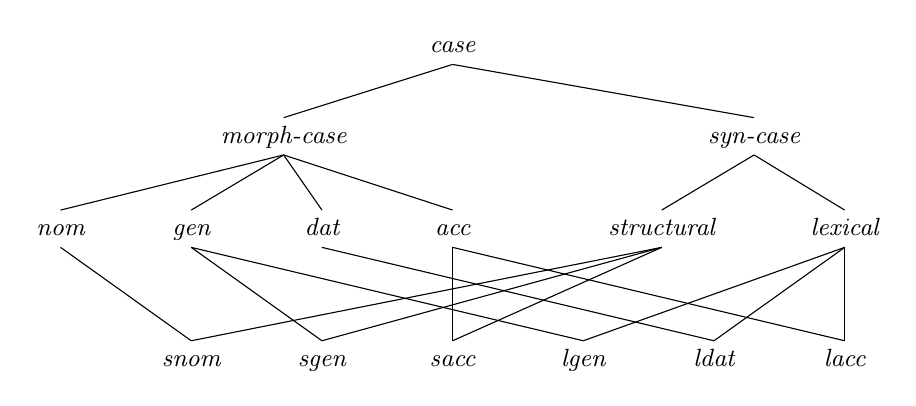
\begin{tikzpicture}[text height=1.5ex,text depth=.25ex,
  % inner sep=2pt,
  node distance=5em,
  baseline=10.75em]\small\it
\node (snom) {snom};
\node (sgen) [right of=snom] {sgen};
\node (sacc) [right of=sgen] {sacc};
\node (lgen) [right of=sacc] {lgen};
\node (ldat) [right of=lgen] {ldat};
\node (lacc) [right of=ldat] {lacc};
\node (acc) [above of=sacc] {acc};
\node (dat) [left of=acc] {dat};
\node (gen) [left of=dat] {gen};
\node (nom) [left of=gen] {nom};
\node (structural) [above of=lgen, xshift=3em] {structural};
\node (lexical) [above of=lacc] {lexical};
\node (morph-case) [above right of=gen] {morph-case};
\node (syn-case) [above right of=structural] {syn-case};
\node (case) [above of=acc, node distance=7em] {case};
\draw (case.south) -- (morph-case.north);
\draw (case.south) -- (syn-case.north);
\draw (morph-case.south) -- (nom.north);
\draw (morph-case.south) -- (gen.north);
\draw (morph-case.south) -- (dat.north);
\draw (morph-case.south) -- (acc.north);
\draw (syn-case.south) -- (structural.north);
\draw (syn-case.south) -- (lexical.north);
\draw (nom.south) -- (snom.north);
\draw (gen.south) -- (sgen.north);
\draw (gen.south) -- (lgen.north);
\draw (dat.south) -- (ldat.north);
\draw (acc.south) -- (sacc.north);
\draw (acc.south) -- (lacc.north);
\draw (structural.south) -- (snom.north);
\draw (structural.south) -- (sgen.north);
\draw (structural.south) -- (sacc.north);
\draw (lexical.south) -- (lgen.north);
\draw (lexical.south) -- (ldat.north);
\draw (lexical.south) -- (lacc.north);
\end{tikzpicture}


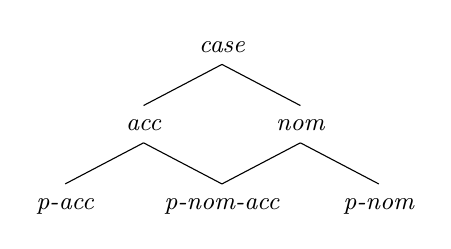
\begin{tikzpicture}[text height=1.5ex,text depth=.25ex,
  % inner sep=2pt,
  node distance=3em,
  baseline=5.25em]\small\it
\node (p-acc) {p-acc};
\node (p-acc1) [right of=p-acc] {};
\node (p-nom-acc) [right of=p-acc1] {p-nom-acc};
\node (p-nom1) [right of=p-nom-acc] {};
\node (p-nom) [right of=p-nom1] {p-nom};
\node (acc) [above of=p-acc1] {acc};
\node (nom) [above of=p-nom1] {nom};
\node (p-nom-acc1) [above of=p-nom-acc] {};
\node (case) [above of=p-nom-acc1] {case};
\draw (case.south) -- (acc.north);
\draw (case.south) -- (nom.north);
\draw (acc.south) -- (p-acc.north);
\draw (acc.south) -- (p-nom-acc.north);
\draw (nom.south) -- (p-nom.north);
\draw (nom.south) -- (p-nom-acc.north);
\end{tikzpicture}

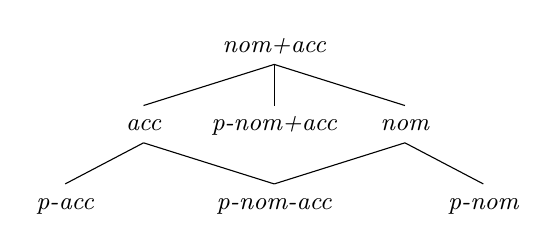
\begin{tikzpicture}[text height=1.5ex,text depth=.25ex,
  % inner sep=2pt,
  node distance=4em,
  baseline=5.25em]\small\it
\node (p-acc) {p-acc};
\node (p-acc1) [right of=p-acc] {};
\node (p-nom-acc) [right of=p-acc1] {p-nom-acc};
\node (p-nom1) [right of=p-nom-acc] {};
\node (p-nom) [right of=p-nom1] {p-nom};
\node (acc) [above of=p-acc1, node distance=3em, xshift=-1em] {acc};
\node (nom) [above of=p-nom1, node distance=3em, xshift=1em] {nom};
\node (p-nom+acc) [above of=p-nom-acc, node distance=3em] {p-nom+acc};
\node (nom+acc) [above of=p-nom+acc, node distance=3em] {nom+acc};
\draw (nom+acc.south) -- (acc.north);
\draw (nom+acc.south) -- (nom.north);
\draw (nom+acc.south) -- (p-nom+acc.north);
\draw (acc.south) -- (p-acc.north);
\draw (acc.south) -- (p-nom-acc.north);
\draw (nom.south) -- (p-nom.north);
\draw (nom.south) -- (p-nom-acc.north);
\end{tikzpicture}


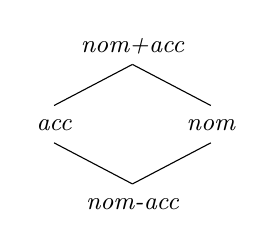
\begin{tikzpicture}[text height=1.5ex,text depth=.25ex,
  % inner sep=2pt,
  node distance=3em,
  baseline=2.5em]\small\it
\node (acc) {acc};
\node (accnom) [right of=acc] {};
\node (nom) [right of=accnom] {nom};
\node (nom-acc) [below of=accnom] {nom-acc};
\node (nom+acc) [above of=accnom] {nom+acc};
\draw (nom+acc.south) -- (acc.north);
\draw (nom+acc.south) -- (nom.north);
\draw (acc.south) -- (nom-acc.north);
\draw (nom.south) -- (nom-acc.north);
\end{tikzpicture}



\hfill\hfill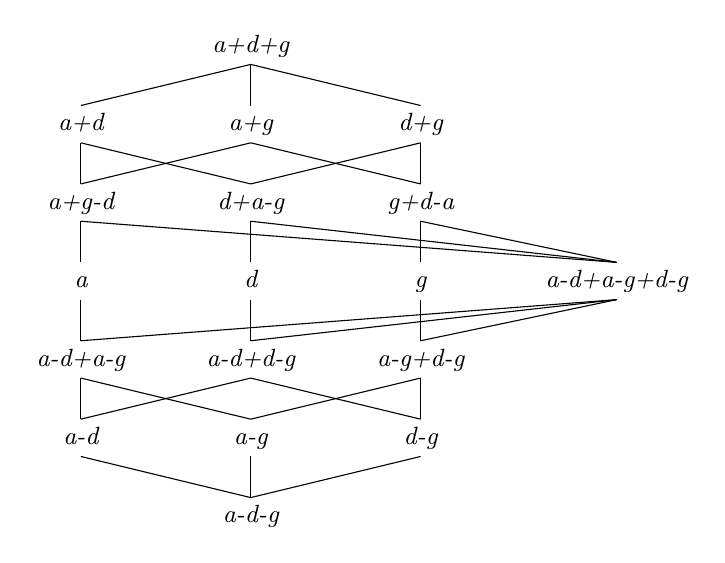
\begin{tikzpicture}[text height=1.5ex,text depth=.25ex,
  % inner sep=2pt,
  node distance=6.5em,
  baseline=8em]\small\it
\node (a) {a};
\node (d) [right of=a] {d};
\node (g) [right of=d] {g};
\node (a-d+a-g+d-g) [right of=g, xshift=1em] {a-d+a-g+d-g};
\node (a+g-d) [above of=a, node distance=3em]  {a+g-d};
\node (d+a-g) [above of=d, node distance=3em] {d+a-g};
\node (g+d-a) [above of=g, node distance=3em] {g+d-a};
\node (a+d) [above of=a+g-d, node distance=3em] {a+d};
\node (a+g) [above of=d+a-g, node distance=3em] {a+g};
\node (d+g) [above of=g+d-a, node distance=3em] {d+g};
\node (a+d+g) [above of=a+g, node distance=3em] {a+d+g};
\node (a-d+a-g) [below of=a, node distance=3em] {a-d+a-g};
\node (a-d+d-g) [below of=d, node distance=3em] {a-d+d-g};
\node (a-g+d-g) [below of=g, node distance=3em] {a-g+d-g};
\node (a-d) [below of=a-d+a-g, node distance=3em] {a-d};
\node (a-g) [below of=a-d+d-g, node distance=3em] {a-g};
\node (d-g) [below of=a-g+d-g, node distance=3em] {d-g};
\node (a-d-g) [below of=a-g, node distance=3em] {a-d-g};
\draw (a+g-d.south) -- (a.north);
\draw (a+g-d.south) -- (a-d+a-g+d-g.north);
\draw (d+a-g.south) -- (d.north);
\draw (d+a-g.south) -- (a-d+a-g+d-g.north);
\draw (g+d-a.south) -- (g.north);
\draw (g+d-a.south) -- (a-d+a-g+d-g.north);
\draw (a+d.south) -- (a+g-d.north);
\draw (a+d.south) -- (d+a-g.north);
\draw (a+g.south) -- (a+g-d.north);
\draw (a+g.south) -- (g+d-a.north);
\draw (d+g.south) -- (d+a-g.north);
\draw (d+g.south) -- (g+d-a.north);
\draw (a+d+g.south) -- (a+d.north);
\draw (a+d+g.south) -- (a+g.north);
\draw (a+d+g.south) -- (d+g.north);
\draw (a.south) -- (a-d+a-g.north);
\draw (d.south) -- (a-d+d-g.north);
\draw (g.south) -- (a-g+d-g.north);
\draw (a-d+a-g.south) -- (a-d.north);
\draw (a-d+a-g.south) -- (a-g.north);
\draw (a-d+d-g.south) -- (a-d.north);
\draw (a-d+d-g.south) -- (d-g.north);
\draw (a-g+d-g.south) -- (a-g.north);
\draw (a-g+d-g.south) -- (d-g.north);
\draw (a-d.south) -- (a-d-g.north);
\draw (a-g.south) -- (a-d-g.north);
\draw (d-g.south) -- (a-d-g.north);
\draw (a-d+a-g+d-g.south) -- (a-d+a-g.north);
\draw (a-d+a-g+d-g.south) -- (a-d+d-g.north);
\draw (a-d+a-g+d-g.south) -- (a-g+d-g.north);
\end{tikzpicture}\hfill\mbox{}



\begin{forest}
%sm edges
[\type{phrase}
	[\textsc{headedness}
		[\type{headed-phrase}
			[\type{head-subject-phrase} [\type{nonfin-head-subj-cx}, name=A2]]
                        [...]			
                        [\type{head-spr-phrase} [\type{noun-poss-cx}, name=B2]]]]			
	[\textsc{clausality}
		[\type{clause}, name=A1]
		[\type{non-clause}, name=B1]]]
\draw (A1.south) -- (A2.north);
\draw (B1.south) -- (B2.north);
\end{forest}



\begin{forest}
%sm edges
[\type{phrase}
	[\textsc{headedness}
		[\type{headed-phrase}
			[\type{head-nonargument-phrase}
				[\type{head-functor-phr} [\type{regular-nominal-phrase}, name=B2]]
				[\type{head-independent-phr}, name=A1]]]]
	[\textsc{clausality}
		[\type{non-clause}
			[\type{nominal-parameter}
			[\type{intersective-modification}, name=B1 [\type{big-mess-phrase}, name=A2]]]]]]
\draw (A1.south) -- (A2.north);
\draw (B1.south) -- (B2.north);
\end{forest}


	\begin{forest}
       [{\type{lexeme}} 
      					[{\fbox{\attrib{part-of-speech}}}
      						[{\type{verb-lx}}, name=A1 
      							[, no edge ]
      							[, no edge ] ] 
      						 [{\type{adj-lx}}]
      						 [{\type{noun-lx}}] 
      						 [{\ldots}]   		
      					] 
      					[{\fbox{\attrib{arg-selection}}} 
      					    [{\type{intr-lx}}
      					 		[{\type{subj-rsg-lx}}
      					 			[{\type{srv-lx}}, name=B1 ]
      					 		]
      					 		[{\ldots}]
      					 	]
      					 	 [{\type{tr-lx}}
      					 		[{\type{obj-rsg-lx}}
      					 			[{\type{orv-lx}}, name=B2 ]
      					 		]
      					 		[{\ldots}]
      					 	]
      					 	[{\ldots}]
      					]  
      	]
      	\draw (A1.south)-- (B1.north);
      	\draw (B2) to [bend left= 6] (A1);
\end{forest}





\begin{tabular}{cccc}
  \tnode{hf}{head-filler-ph} & \tnode{itrr}{interr-cl} & \tnode{rel}{rel-cl} & \tnode{decl}{decl-cl}\\[2em]

  \tnode{whi}{wh-interr-cl} & \tnode{whr}{wh-rel-cl} & \tnode{top}{top-cl} & \tnode{the}{the-cl}
\end{tabular}



\psset{linewidth=.5pt,angleA=-90,angleB=90,arm=0pt,nodesepA=2pt}

\bcdiag{hf}{whi}
\bcdiag{itrr}{whi}
\bcdiag{hf}{whr}
\bcdiag{rel}{whr}
\bcdiag{hf}{top}
\bcdiag{decl}{top}
\bcdiag{hf}{the}
\bcdiag{decl}{the}

\begin{tabular}{ccccc}
\multicolumn{2}{c}{\tnode{hf}{head-filler-ph}} & \tnode{itrr}{interr-cl} & \tnode{rel}{rel-cl} & \tnode{decl}{decl-cl}\\[1em]
\tnode{std}{standard-head-fill-ph}\\[1.5em]
\tnode{whi}{wh-interr-cl} & \multicolumn{2}{c}{\tnode{whr}{wh-rel-cl}} & \tnode{top}{top-cl} & \tnode{the}{the-cl}\\[1.5em]
&  \tnode{fwh}{fin-wh-rel-cl} & \tnode{iwh}{inf-wh-rel-cl}


\end{tabular}



\psset{linewidth=.5pt,angleA=-90,angleB=90,arm=0pt,nodesepA=2pt}
  
\bcdiag{hf}{std}
\bcdiag{std}{whi}
\bcdiag{itrr}{whi}
\bcdiag{std}{whr}
\bcdiag{rel}{whr}
\bcdiag{std}{top}
\bcdiag{decl}{top}
\bcdiag{hf}{the}
\bcdiag{decl}{the}
\bcdiag{whr}{fwh}
\bcdiag{whr}{iwh}


  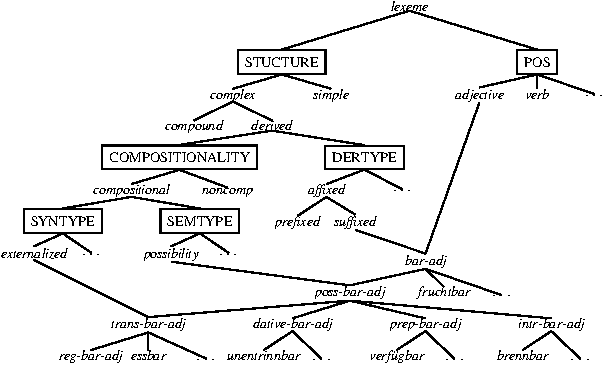
\includegraphics[scale=1.2]{figures/Riehemann-crop.pdf}


  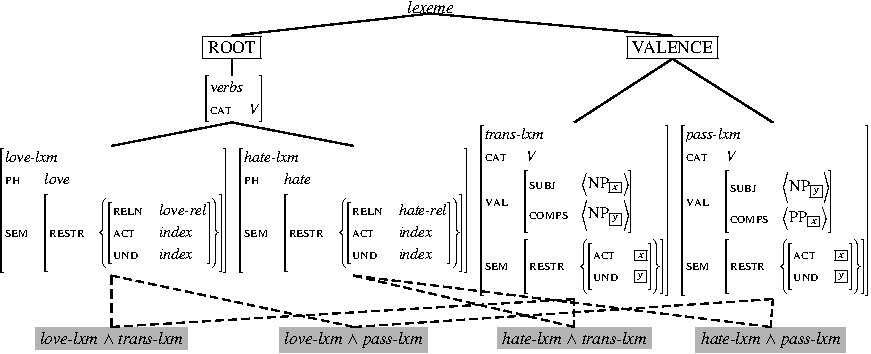
\includegraphics[scale=.84]{figures/OTC-crop.pdf}

  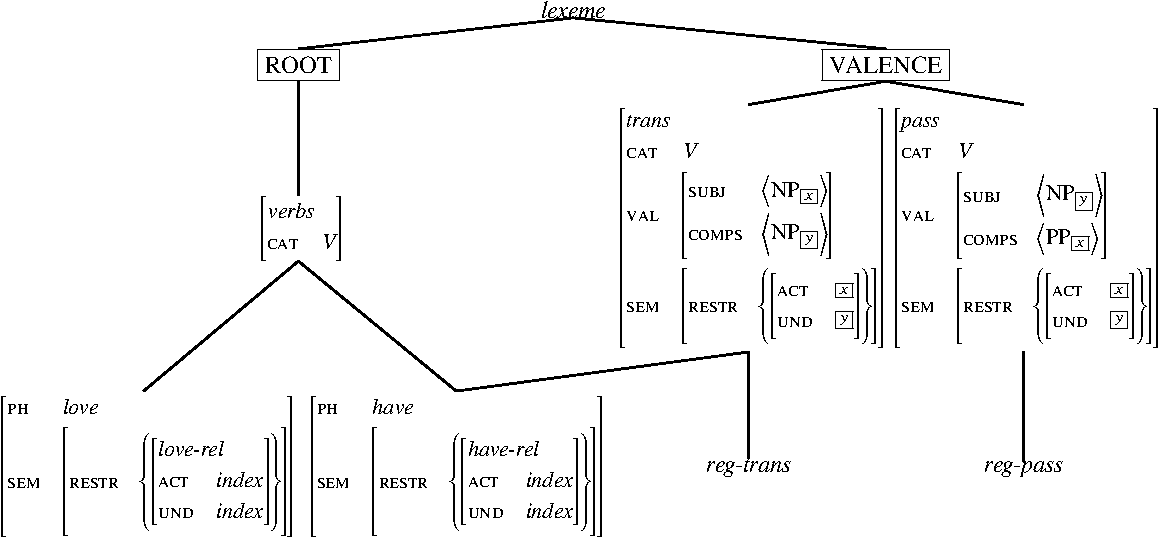
\includegraphics[scale=.63]{figures/pretyping-crop.pdf}



\begin{forest}
[\emph{verb-infl}
	[2ND-SLOT,draw
    	[\emph{1sg},name=1sg
    		[\emph{1sg-pos}]
    	]
    	[\emph{3pl}]
   ]
	[1ST-SLOT,draw
		[\emph{neg}
			[\emph{1sg-neg},name=neg]
			[\emph{¬1sg-neg}]
		]
		[\emph{pos}]
	]
	[3RD-SLOT,draw
		[\emph{pst}
			[\emph{pos-pst}]
			[\emph{neg-pst}]
		]
		[\emph{fut}]
	]
]
\draw (1sg.south) to (neg.north);
\end{forest}



%% This does not compile ....

\scalebox{.8}{%
\begin{forest}for tree={l=2cm}
[\emph{realisation-rule}
	[MORPHOTACTICS,draw, name=morph
		[{\begin{avm}
			\[
			mud & \{\normalfont\textit{agr} \}\\
			ms & \{ \[\asort{pid}
			cat & verb\], ...\}\\
			mph & \< \[pc & $-4$\]\> \]
		\end{avm}}, name= 1, tier=word]
		[{\begin{avm}
			\[mud & \{\normalfont\textit{agr}\}\\
			 ms & \{ \[\asort{pid}
			cat & \[\asort{adj}
			type & A\]\], ...\}\\
			mph & \< \[pc & -1\]\>\]
		\end{avm}}, name=2, tier=word]
	]
	[EXPONENCE,draw
		[QUAL,draw, name=qual
			[{\begin{avm}
				\[mud & \{ \[\normalfont\textit{agr}\\cl & 7\]\}\\
				mph & \< ... \[ph & \<\normalfont ca\>\\
				pc & $-1$ $\vee$ $-2$
				\] ... \>\]
			\end{avm}}, tier=word]
			[\dots]
		]
		[CONC,draw, name=conc
			[{\begin{avm}
				\[mud & \{ \[\normalfont\textit{agr}\\cl & 7\]\}\\
				mph & \< ... \[ph & \<\normalfont ci\>\\
				pc & $-1$ $\vee$ $-4$
				\] ... \>\]
			\end{avm}}, tier=word]
			[\dots]
		]
	]
]
%% sorry this is an ugly workaround but even on stackexchange, no one could help me :/
\node[below of=morph, node distance= 8cm](3){%
	{\begin{avm}
			\[mud & \{\normalfont\textit{agr}\}\\
			ms & \{ \[\asort{pid}
			cat & \[\asort{adj}
			type & B\]\], ...\}\\
			mph & \<\[pc & $-2$\], \[pc & $-1$\]\>\]
	\end{avm}}%
};
\draw (1.north) to (qual.south);
\draw (2.north) to (conc.south);
\draw (3.north) to (morph.south);
\end{forest}
}    


  \begin{tabular}{lcc}
    \rnode{u1}{\textsc{beak}} & \rnode{u2}{\textsc{gen}} & \rnode{u3}{\textsc{pl}}\\[2ex]
    \rnode{l1}{nokk} & \rnode{l2}{-a} & \rnode{l3}{-de}
  \end{tabular}
      \psset{angleA=-90,angleB=90,arm=0pt,linewidth=.5pt}

      \ncdiag{u1}{l1} \ncdiag{u1}{l2} \ncdiag{u2}{l1} \ncdiag{u2}{l3}
      \ncdiag{u3}{l1} \ncdiag{u3}{l2} \ncdiag{u3}{l3}


\begin{forest}
[\emph{realisation-rule}
	[SHAPE,draw
		[{\begin{avm}
			\[ mph & \{\[ph &  \<\normalfont ni\>\]\}\\
			mud & \{\[per & 1\\ num & sg\]\}
			\]
		\end{avm}}, name=1
			[{\begin{avm}
				\[ mph & \{\[ph &  \<\normalfont ni\>\\ pc & 2\]\}\\
				mud & \{ \[\asort{subj} per & 1\\ num & sg\] \}
				\]
			\end{avm}}, name=a, no edge, tier=word, l=3cm]
		]
		[{\begin{avm}
			\[ mph & \{\[ph &  \<\normalfont wa\>\]\}\\
			mud & \{\[per & 3\\ num & pl\]\}
			\]
		\end{avm}}, name=2
			[{\begin{avm}
				\[ mph & \{\[ph &  \<\normalfont wa\>\\ pc & 5\]\}\\
				mud & \{ \[\asort{obj} per & 3\\ num & pl\] \}
				\]
			\end{avm}}, name=b, no edge, tier=word, l=3cm]
		]
	]
	[POSITION,draw
		[{\begin{avm}
			\[ mph & \{\[pc & 2\]\}\\
			mud & \{subj\}
			\]
		\end{avm}}, name=3
			[{\begin{avm}
				\[ mph & \{\[ph &  \<\normalfont wa\>\\ pc & 2\]\}\\
				mud & \{ \[\asort{subj} per & 3\\ num & pl\] \}
				\]
			\end{avm}}, name=c, no edge, tier=word, l=3cm]
		]
		[{\begin{avm}
			\[ mph & \{\[pc & 5\]\}\\
			mud & \{ obj \}
			\]
		\end{avm}}, name=4
			[{\begin{avm}
				\[ mph & \{\[ph &  \<\normalfont ni\>\\ pc & 5\]\}\\
				mud & \{\[\asort{obj} per & 1\\ num & sg\]\}
				\]
			\end{avm}}, name=d, no edge, tier=word, l=3cm]
		]
	]
]
\draw[dashed] (1.south) to (a.north);
\draw[dashed] (1.south) to (d.north);
\draw[dashed] (2.south) to (b.north);
\draw[dashed] (2.south) to (c.north);
\draw[dashed] (3.south) to (c.north);
\draw[dashed] (3.south) to (a.north);
\draw[dashed] (4.south) to (b.north);
\draw[dashed] (4.south) to (d.north);
\end{forest}






}


\end{document} 

%%%%%%%%%%%%%%%%%%%%%%%%%%%%%%%%%%%%%%%%%%%%%%%%%%%% 
%%%                  END                         %%% 
%%%%%%%%%%%%%%%%%%%%%%%%%%%%%%%%%%%%%%%%%%%%%%%%%%%% 
